\section{Statistical Approaches}


\begin{frame}{Statistical Approaches}
	\begin{itemize}
		\item \textbf{Assumption:} Objects in a data set are \textbf{\color{airforceblue}generated by a stochastic process} (a generative model).
		\item \textbf{Idea:} Learn a generative model fitting the given data set, and then identify the objects in low-probability regions of the model as outliers.
		\item \textbf{Methods divided into two categories:}
	\end{itemize}
	\vspace*{-2em}
	\begin{columns}
		\begin{column}{0.5\textwidth}
			\begin{center}
				\textbf{Parametric Methods}
			\end{center}
			\vspace*{-1.2em}
			\begin{itemize}
				\item Assumes that the normal data is generated by a parametric distribution with parameter $\theta$.
				\item The probability density function of the parametric distribution $f(x, \theta)$ gives the probability that object $x$ is generated by the distribution.
				\item Small values indicate potential outlier.
			\end{itemize}
		\end{column}
		\begin{column}{0.5\textwidth}
			\pause
			\begin{center}
				\textbf{Non-Parametric Methods}
			\end{center}
			\vspace*{-1.2em}
			\begin{itemize}
				\item Do not assume an a-priori statistical model and determine the model from the input data.
				\item Not completely parameter-free, but consider number and nature of the parameters to be flexible and not fixed in advance.
				\item \textbf{Examples:} \textbf{\color{airforceblue}histogram} and kernel-density estimation.
			\end{itemize}
		\end{column}
	\end{columns}
\end{frame}


\begin{frame}{Parametric Methods I: Detection Based on Normal Distribution}
	% TODO: add plot for visual motivation
	\begin{itemize}
		\item \textbf{Univariate data:} A data set involving \textit{only one attribute} or variable.
		\item \textbf{Assumption:} Data are generated from a normal distribution.
		\item \textbf{Learn the parameters from the input data, and identify the points with low probability as outliers.}
	\end{itemize}
	\vspace*{0.5em}
	\textbf{Example:} Assume data follows a \textbf{normal distribution}.
	\begin{itemize}
		\item \underline{Recall:} normal distribution $\mathcal{N}(\mu, \sigma)$
		      \begin{itemize}
			      \item Characterized by two parameters: mean $\mu$, and standard deviation $\sigma$.
			      \item Probability density functin: $f(x)=\frac{1}{\sqrt{2\pi \sigma^2}} {\rm e}^{-\frac{(x-\mu)^2}{2\sigma^2}}$.
		      \end{itemize}
		\item \textbf{\color{faugray}Idea:} Estimate parameters $\mu$ and $\sigma$ so that normal distribution fits data as close as possible.
		\item \textbf{Question:} How to estimate these parameters? $\rightarrow$ \textit{\color{faugray}Maximum likelihood method.}
	\end{itemize}
\end{frame}



\begin{frame}{Excursus: Maximum Likelihood Estimation I}
	\begin{block}{Maximum Likelihood Estimation}
		\textit{Maximum Likelihood Estimation} (MLE) estimates \textit{parameters} of an assumed probability distribution such that the \textit{distribution fits the data as closely as possible}.
	\end{block}
	\begin{itemize}
		\item \textbf{Likelihood function} $\mathcal{L}(\theta|X)$ with
		      \begin{itemize}
			      \item parameter space $\theta$ and
			      \item observed data $X=\{x_1, x_2, \dots, x_n\}$
		      \end{itemize}
		      describes the joint probability of observed data as a function of the parameters of the assumed distribution.
		      \begin{itemize}
			      \item Frequently assumed distribution: Gaussian (normal) distribution $\mathcal{N}(\mu, \sigma)$.
			      \item Thus, the likelihood function $\mathcal{L}(\theta|X)$ with parameter space $\theta=\{\mu, \sigma\}$ is the Gaussian process:
			            \begin{equation*}
				            \mathcal{L}(\theta|X)=\mathcal{L}(\mu, \sigma|x_1, \dots, x_n) = \prod\nolimits_{i=1}^n \frac{1}{\sqrt{2\pi \sigma^2}} {\rm e}^{-\frac{(x_i-\mu)^2}{2\sigma^2}}
			            \end{equation*}
		      \end{itemize}
		\item Find good estimates for $\theta$ such that $\widehat{\theta} = \argmax_{\theta} \mathcal{L}(\theta|X)$.
	\end{itemize}
\end{frame}


\begin{frame}{Excursus: Maximum Likelihood Estimation II}
	\begin{itemize}
		\item In the case of a Gaussian distribution: find estimates for $\mu$ and $\sigma$ such that
		      \begin{align*}
			      \widehat{\mu}    & = \textstyle\argmax_{\mu} \mathcal{L}(\theta|X),   \\
			      \widehat{\sigma} & = \textstyle\argmax_{\sigma} \mathcal{L}(\theta|X)
		      \end{align*}
		\item \textbf{General procedure:}
		      \begin{enumerate}
			      \item Generate two derivatives, with respect to $\mu$ and $\sigma$, respectively.
			      \item Solve each equation by setting them equal to zero.
		      \end{enumerate}
		\item Instead of taking the derivative directly, we take the log of the likelihood function as this makes it easier to take derivatives.
		      \begin{equation*}
			      \ln{\mathcal{L}(\theta|x_1, \dots, x_n)}=\ln{\mathcal{L}(\mu, \sigma|x_1, \dots, x_n)}= \ln{\bigg({\textstyle\prod\nolimits_{i=1}^n} \frac{1}{\sqrt{2\pi \sigma^2}} {\rm e}^{-\frac{(x_i-\mu)^2}{2\sigma^2}}\bigg)}
		      \end{equation*}
		      \begin{itemize}
			      \item Logarithm is monotonically increasing, thus satisfying $\argmax_{\theta} \; \ln(\mathcal{L}(\theta|X)) = \text{argmax}_{\theta} \; \mathcal{L}(\theta|X)$.
			      \item Logarithm turns multiplication $\prod$ into addition $\sum$ making derivatives easier to compute.
		      \end{itemize}
	\end{itemize}
\end{frame}
% TODO: MLE easily motivated and explained visually. Mabye insert plots similarly to ML hands-on book p. 269

\begin{frame}{Excursus: Maximum Likelihood Estimation III}
	\begin{enumerate}
		\setcounter{enumi}{-1}
		\item Transform equation:
		      \vspace*{-1em}
		      \begin{equation*}
			      \ln \mathcal{L}(\mu, \sigma | x_1, \dots, x_n) = \ln{\bigg({\textstyle\prod\nolimits_{i=1}^n} \frac{1}{\sqrt{2\pi \sigma^2}} {\rm e}^{-\frac{(x_i-\mu)^2}{2\sigma^2}}\bigg)}= -\frac{n}{2}\ln{2\pi}-\frac{n}{2}\ln{\sigma^2}-\frac{1}{2\sigma^2}\textstyle\sum\nolimits_{i=1}^n (x_i - \mu)^2
		      \end{equation*}
		\item To estimate parameters, take the partial derivative with respect to $\mu$ and $\sigma$:
		      \vspace*{-1em}
		      \begin{align*}
			      \textstyle\frac{\partial}{\partial \mu}\ln{(\mathcal{L}(\mu, \sigma|x_1, \dots, x_n))}    & = \frac{1}{\sigma^2} \sum_{i=1}^n (x_i -\mu)                            \\
			      \textstyle\frac{\partial}{\partial \sigma}\ln{(\mathcal{L}(\mu, \sigma|x_1, \dots, x_n))} & =-\textstyle\frac{n}{\sigma}+\frac{1}{\sigma^3}\sum_{i=1}^n (x_i-\mu)^2
		      \end{align*}
		\item Then, by setting these quation equals zero, we derive the following likelihood estimates:
		      \begin{center}
			      mean $\widehat{\mu}=\frac{1}{n}\sum\nolimits_{i=1}^n x_i$ \hspace{3em} standard deviation $\widehat{\sigma}=\sqrt{\frac{1}{n}\sum\nolimits_{i=1}^n (x_i-\mu)^2}$
		      \end{center}
		      % TODO: proof in appendix or discuss in lecture?
	\end{enumerate}
	\begin{flushright}
		{\color{gray}Refer to appendix for proof.}
	\end{flushright}
\end{frame}

\begin{frame}{Parametric Methods I: Detection Based on Normal Distribution (2)}
	\textbf{Example:}
	\begin{itemize}
		\item Average yearly temperatures: $\{24.0, 28.9, 28.9, 29.0, 29.1, 29.1, 29.2, 29.2, 29.3, 29.4\}$.
		      % TODO: plot data?
		\item For these data with $n = 10$, we have
		      \begin{align*}
			      \widehat{\mu}=28.61, \quad \widehat{\sigma}=\sqrt{2.29}=1.51.
		      \end{align*}
		\item Then the most deviating value $24.0$ is $4.61$ away form the estimated mean.
		\item \textbf{Recall:} $\mu \pm 3\sigma $ contains $99.7\%$ of the data under the assumption of normal distribution.
		\item $\mu \pm 3\sigma$\pause~$ \Leftrightarrow \mu - 3\sigma \leq x \le \mu + 3\sigma$\pause~$ \Leftrightarrow \frac{\mu - x}{\sigma} \leq 3 \leq \frac{\mu - x}{\sigma}$
		\item Plugging in the minimum value ($24.0$) into the equation yields $\frac{\mu-x}{\sigma} = \frac{28.61 - 24}{1.51} =\frac{4.61}{1.51}  =  3.04  >  3$
		\item Probability that $24.0$ is generated by a normal distribution is less than $0.15\%$.
		      \begin{itemize}
			      \item Each \emph{tail} to the left and to the right of the $99.7\%$ has $0.15\%$.
		      \end{itemize}
		\item Hence, $24.0$ identified as an outlier.
	\end{itemize}
\end{frame}


\begin{frame}{Parametric Methods I: The Grubbs' Test\footnote{Named after Frank E. Grubbs.}}
	\begin{block}{Grubbs' Test}
		The \textit{Grubbs' Test} is a statistical test to detect outlier in a \underline{univariate} data set under the assumption that this data set follows a normal distribution. Grubbs' Test is also known as \textit{maximum normed residual test}.
	\end{block}
	\begin{itemize}
		\item Postulates following hypotheses:
		      \begin{itemize}
			      \item $H_0:$ Data set contains no outliers.
			      \item $H_a:$ Data set contains exactly one outlier.
		      \end{itemize}
		\item For a data set $\{x_1, x_2, \dots, x_n\}$ compute the \textbf{Grubbs' test statistic}:  $G = \frac{\max\vert x_i - \overline{x}\vert}{s}$,\\
		      with sample mean $\overline{x}$ and  sample standard deviation $s$.

		\item The two-sided test with significance level $\alpha$ to reject the null hypothesis is as follows:
		      \begin{columns}
			      \begin{column}{0.3\columnwidth}
				      \vspace*{-1em}
				      \begin{flushright}
					      $G > \frac{N-1}{\sqrt{N}} \sqrt{\frac{t^2_{\frac{\alpha}{2N},N-2}}{N-2 + t^2_{\frac{\alpha}{2N},N-2}}}$
				      \end{flushright}
				      \vspace*{0.5em}
			      \end{column}
			      \begin{column}{0.6\columnwidth}
				      where $t^2_{\frac{\alpha}{2N},N-2}$ is the value taken by a $t$-distribution at a significance level of $\frac{\alpha}{2N}$,\\ and $N$ is the number of objects in the data set.
			      \end{column}
		      \end{columns}

	\end{itemize}
\end{frame}


\begin{frame}{Parametric Methods II: Detection of Multivariate Outliers}
	\begin{itemize}
		\item \textbf{Multivariate data}: A data set involving \textbf{\color{faugray}two or more attributes} or variables.
		\item Univariate outlier detection methods can be extended to the multivariate case.
		\item \textbf{Central Idea:} Transform the multivariate outlier-detection task into a univariate outlier-detection problem.
		\item Methods include but not limited to:
		      \begin{enumerate}
			      \item Mahalanobis distance.
			      \item $\chi^2$ statistic
		      \end{enumerate}
	\end{itemize}
	\begin{alertblock}{Beware: Term ``Multivariate'' Defined Differently Throughout Disciplines}
		Depending on the discipline of the paper you may find yourself reading, the term multivariate data, though, maybe misleading. For instance, in probability and statistics, a \textit{multivariate random variable} is a \underline{column vector} $X=\{x_1, x_2, \dots, x_n\}$, i. e. univariate data. However, a \textit{multivariate time series} contains \underline{multiple univariate} time series (column vectors).
	\end{alertblock}
\end{frame}


\begin{frame}{Parametric Methods II: Mahalanobis Distance and $\chi^2$ Statistic}
	\vspace*{-2em}
	\begin{columns}[t]
		\begin{column}{0.5\textwidth}
			\begin{center}
				\textbf{Mahalanobis Distance}
			\end{center}
			\vspace*{-1em}
			\begin{itemize}
				\item Measures the distance between an object $\mathbf{x}$ and the data set's distribution.
				\item Defined as
				      \begin{align*}
					      \text{MD}(\mathbf{x}) = \sqrt{(\mathbf{x} - \mathbf{\overline{x}})^T \mathbf{C}^{-1} (\mathbf{x} - \mathbf{\overline{x}})}
				      \end{align*}
				      with mean $\mathbf{\overline{x}}$, and covariance matrix $\mathbf{C}$, and $\mathbf{x}=(x_1, x_2, \dots, x_n)$ where $x_i$ is a column vector at position $i$.
				\item Use the Grubbs' test on this measure to detect outliers.
			\end{itemize}
		\end{column}

		\begin{column}{0.5\textwidth}
			\begin{center}
				\textbf{$\chi^2$ Statistic}
			\end{center}
			\vspace*{-1em}
			\begin{itemize}
				\item Captures multivariate outliers under the assumption of a normal distribution.
				\item For a data set $\mathbf{x}=(x_1, x_2, \dots, x_n)$, $\chi^2$ statistic is defined as:
				      \begin{align*}
					      \chi^2 = \sum_{i=1}^n \frac{x_i - \overline{x}}{\overline{x}}
				      \end{align*}
				\item If $\chi^2$ statistic is large, then $\mathbf{x}_i$ is an outlier.
			\end{itemize}
		\end{column}
	\end{columns}
\end{frame}

% TODO: Add book author name in footnote
\begin{frame}{Parametric Methods III: Using Mixture of Parametric Distributions}
	\tikzoverlay at (11cm,0.5cm) {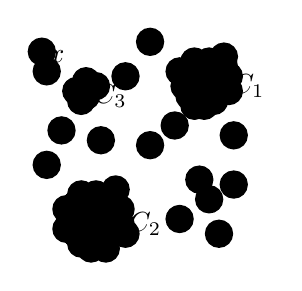
\begin{tikzpicture}[
		scale=0.25,
		region/.style={
				draw=black,
				shape=circle,
				dashed
			},
		mycircle/.style={
				draw,
				>=latex,
				thick,
				shape=circle,
				fill=black,
				minimum width=0.3em
			},
	]
	\node [mycircle] (1) at (-9.75, -10.25) {};
	\node [mycircle] (3) at (-10.25, -11.5) {};
	\node [mycircle] (4) at (-9.75, -11.75) {};
	\node [mycircle] (5) at (-9, -12.5) {};
	\node [mycircle] (6) at (-8.5, -10.75) {};
	\node [mycircle] (7) at (-10, -10.75) {};
	\node [mycircle] (9) at (-8.5, -11) {};
	\node [mycircle] (10) at (-9, -11) {};
	\node [mycircle] (11) at (-9.25, -11.5) {};
	\node [mycircle] (12) at (-8.75, -11.75) {};
	\node [mycircle] (14) at (-9.5, -10.75) {};
	\node [mycircle] (15) at (-10.25, -10.5) {};
	\node [mycircle] (16) at (-9.75, -11.25) {};
	\node [mycircle] (19) at (-7.75, -11) {};
	\node [mycircle] (20) at (-7.25, -11.75) {};
	\node [mycircle] (21) at (-8.25, -12.5) {};
	\node [mycircle] (22) at (-8.25, -10.25) {};
	\node [mycircle] (25) at (-8, -11.75) {};
	\node [mycircle] (26) at (-8.25, -12) {};
	\node [mycircle] (27) at (-7.5, -11.25) {};
	\node [mycircle] (28) at (-8.75, -9.75) {};
	\node [mycircle] (30) at (-4.5, -11) {};
	\node [mycircle] (31) at (-3, -10) {};
	\node [mycircle] (34) at (-7.5, -10.5) {};
	\node [mycircle] (36) at (-3.5, -9) {};
	\node [mycircle] (37) at (-3.25, -5.25) {};
	\node [mycircle] (38) at (-2.5, -11.75) {};
	\node [mycircle] (39) at (-1.75, -9.25) {};
	\node [mycircle] (41) at (-3, -3) {};
	\node [mycircle] (44) at (-3.75, -5.25) {};
	\node [mycircle] (45) at (-2, -3.75) {};
	\node [mycircle] (47) at (-2.75, -4.25) {};
	\node [mycircle] (53) at (-1.75, -6.75) {};
	\node [mycircle] (56) at (-4.75, -6.25) {};
	\node [mycircle] (57) at (-2.75, -5) {};
	\node [mycircle] (58) at (-4.5, -3.5) {};
	\node [mycircle] (59) at (-3.75, -3) {};
	\node [mycircle] (61) at (-2.5, -3.75) {};
	\node [mycircle] (65) at (-3.25, -4.5) {};
	\node [mycircle] (66) at (-3.75, -3.75) {};
	\node [mycircle] (67) at (-3.25, -4.75) {};
	\node [mycircle] (68) at (-4.25, -4.25) {};
	\node [mycircle] (69) at (-3.75, -4.25) {};
	\node [mycircle] (70) at (-6, -7.25) {};
	\node [mycircle] (71) at (-9.5, -5) {};
	\node [mycircle] (72) at (-4, -4.75) {};
	\node [mycircle] (74) at (-9.25, -4) {};
	\node [mycircle] (78) at (-9.25, -4.75) {};
	\node [mycircle] (79) at (-9.75, -4.5) {};
	\node [mycircle] (80) at (-8.75, -4.25) {};
	\node [mycircle] (81) at (-10.5, -6.5) {};
	\node [mycircle] (82) at (-11.25, -8.25) {};
	\node [mycircle] (83) at (-8.5, -7) {};
	\node [mycircle] (87) at (-2.25, -2.75) {};
	\node [mycircle] (89) at (-9.5, -12.25) {};
	\node [mycircle] (93) at (-7.75, -9.5) {};
	\node [mycircle] (95) at (-3.25, -3.75) {};
	\node [mycircle] (97) at (-2, -4.5) {};
	\node [mycircle] (100) at (-2.25, -3.25) {};
	\node [mycircle] (101) at (-11.25, -3.5) {};
	\node [mycircle] (103) at (-11.5, -2.5) {};
	\node [mycircle] (104) at (-7.25, -3.75) {};
	\node [mycircle] (105) at (-6, -2) {};
	\node [mycircle] (106) at (-9.5, -9.75) {};
	\node [mycircle] (107) at (-9.25, -10.25) {};
	\node (109) at (-1, -4.25) {$C_1$};
	\node (112) at (-8, -4.75) {$C_3$};
	\node (113) at (-6.25, -11.25) {$C_2$};
	\node (114) at (-10.75, -2.75) {$x$};
\end{tikzpicture}
};
	\begin{itemize}
		\item Assuming data follows a normal distribution is too simple for complex\\ data distributions.
		\item Right figure: The objects between the two clusters cannot be captured\\ as outliers since they are close to the estimated mean.
		\item \textbf{Assume data is generated by {\color{airforceblue}two normal distributions.}}
		      \begin{itemize}
			      \item For any object $\mathbf{x}$ in the data set, the probability that $\mathbf{x}$ is generated by the mixture of the two distributions $\mathcal{N}_1(\mu_1, \sigma_1)$ and $\mathcal{N}_2(\mu_2, \sigma_2)$ is given by
			            \begin{align*}
				            \text{P}(\mathbf{x} \; \vert \; \mathcal{N}_1, \mathcal{N}_2) = f_{\mathcal{N}_1}(\mathbf{x} \; \vert \; \mu_1, \sigma_1) + f_{\mathcal{N}_2}(\mathbf{x} \; \vert \; \mu_2, \sigma_2),
			            \end{align*}
			            where $f_{\mathcal{N}_1}$ and $f_{\mathcal{N}_1}$ are the probability density functions of $\mathcal{N}_1$ and $\mathcal{N}_2$, respectively.
			      \item Use expectation-maximization (EM) algorithm\footnote{Expectation-maximization algorithm is not covered in this lecture. If you are interested, you may take a look at chapter 11 of our reference book titled \citetitle{han2011}.} to learn the parameters $\mu_1, \sigma_1, \mu_2, \sigma_2$ from the data.
			      \item An object $\mathbf{x}$ is an outlier if it does not belong to any cluster.
		      \end{itemize}
	\end{itemize}
\end{frame}


\begin{frame}{Non-Parametric Methods: Detection Using Histogram I}
	\textit{Non-parametric methods} make fewer assumptions about the data, and thus are applicable in more scenarios.\\\bigskip

	\textbf{Outlier detection using histograms:}
	\begin{columns}
		\begin{column}{0.7\textwidth}
			\vspace*{-1em}
			\begin{enumerate}
				\item Construct histogram
				\item Detect outiler by checking objects against the histogram and determine if is normal or not.\\
				      \textbf{Example:} A transaction with the amount of $\$7,500$ is an outlier, since only $0.2\%$ \\ of the transactions have an amount higher than $\$5,000$.
			\end{enumerate}
		\end{column}
		\begin{column}{0.3\textwidth}
			\begin{figure}
				\centering
				\includegraphics[width=\textwidth]{img/histogram8.png}
			\end{figure}
		\end{column}
	\end{columns}
\end{frame}


\begin{frame}{Non-Parametric Methods: Detection Using Histogram II}
	\textbf{Problem:}
	\begin{itemize}
		\item Hard to \textbf{\color{airforceblue}choose an appropriate bin size} for histogram.
		\item Too small bin size $\rightarrow$ normal objects in empty/rare bins, false positive.
		\item Too big bin size $\rightarrow$ outliers in some frequent bins, false negative.
	\end{itemize}
	\vspace*{1em}
	\textbf{Alternatively:} Estimate probability density function with \textbf{Kernel Density Estimation} (KDE)
	\begin{itemize}
		\item Given: Univariate data set $X=\{x_1, x_2, \dots, x_n\}$ that is drawn i.\,i.\,d (independent and identically distributed)
		\item Its \underline{kernel density estimate} is $\hat{f}_h(x)=\frac{1}{n}\sum_{i=1}^n K_h(x-x_i) = \frac{1}{nh}\sum_{i=1}^n K(\frac{x-x_i}{h})$, where
		      \begin{itemize}
			      \item $\hat{f}$ is the density function to be estimated,
			      \item $h>0$ is a smoothing parameter, also called \textit{bandwidth}, corresponds to the bin width of the histogram. If too small, the curve gets too rough, if too large, shape of $\hat{f}$ is too washed out.
			      \item $K$ is the kernel, a non-negative function, typically standard Gaussian function with $\mu=0$ and $\sigma=1$.
			      \item $K_h$ is the scaled kernel $K_h(x)=\frac{1}{h} K(\frac{x}{h})$
		      \end{itemize}
	\end{itemize}
	% TODO: Add plot of KDE?
\end{frame}
